\documentclass[UTF8,a4paper,12pt]{ctexbook} 

 \usepackage{graphicx}%学习插入图
 \usepackage{verbatim}%学习注释多行
 \usepackage{booktabs}%表格
 \usepackage{geometry}%图片
 \usepackage{amsmath}
 \usepackage{amssymb}
 \usepackage{listings}%代码
 \usepackage{xcolor}  %颜色
 \usepackage{enumitem}%列表格式
 \usepackage{tcolorbox}
 \usepackage{algorithm}  %format of the algorithm
 \usepackage{algorithmic}%format of the algorithm
 \usepackage{multirow}   %multirow for format of table
 \usepackage{tabularx} 	%表格排版格式控制
 \usepackage{array}	%表格排版格式控制
 \usepackage{hyperref} %超链接 \url{URL}
\CTEXsetup[format+={\flushleft}]{section}


\geometry{left=1.6cm,right=1.8cm,top=2cm,bottom=1.7cm} %设置文章宽度

\pagestyle{plain} 		  %设置页面布局
\author{\kaishu 郑华}
\title{\textbf{C++\_Boost 总结}}

\newcommand{\Code}[1]{$\textbf{清单:}#1\ $}
 %代码效果定义
 \definecolor{mygreen}{rgb}{0,0.6,0}
 \definecolor{mygray}{rgb}{0.5,0.5,0.5}
 \definecolor{mymauve}{rgb}{0.58,0,0.82}
 \lstset{ %
 	backgroundcolor=\color{white},   % choose the background color
 	basicstyle=\footnotesize\ttfamily,        % size of fonts used for the code
 	%stringstyle=\color{codepurple},
 	%basicstyle=\footnotesize,
 	%breakatwhitespace=false,         
 	%breaklines=true,                 
 	%captionpos=b,                    
 	%keepspaces=true,                 
 	%numbers=left,                    
 	%numbersep=5pt,                  
 	%showspaces=false,                
 	%showstringspaces=false,
 	%showtabs=false,        
 	columns=fullflexible,
 	breaklines=true,                 % automatic line breaking only at whitespace
 	captionpos=b,                    % sets the caption-position to bottom
 	tabsize=4,
 	commentstyle=\color{mygreen},    % comment style
 	escapeinside={\%*}{*)},          % if you want to add LaTeX within your code
 	keywordstyle=\color{blue},       % keyword style
 	stringstyle=\color{mymauve}\ttfamily,     % string literal style
  	frame=single,					%tb top and bottom; L left double line
  	xleftmargin=.06\textwidth, 
  	%xrightmargin=.1\textwidth,
 	rulesepcolor=\color{red!20!green!20!blue!20},
 	% identifierstyle=\color{red},
 	language=c++,
 }
 %正文排版开始
 \begin{document} 
 	\maketitle
	\tableofcontents
\newpage 

\chapter{学习-荐}
	\section{陈硕谈Boost}
		\verb|noncopyable、scoped_ptr、 static_assert|
		
		\verb|function/bind|
		
		\verb|shared_ptr|

\chapter{安装}
	 \section{安装步骤}
		 \subparagraph{1.下载 Boost库}
		 \subparagraph{2.解压到指定文件夹,如D:Boost}
		 \subparagraph{3.执行批处理 文件booststrap.bat 文件}
		 \subparagraph{4.点击执行新生成的bjam.exe 文件,大概10分钟}
		 \subparagraph{5.新建一个win32控制台空项目测试}
		 \subparagraph{6.解决方案配置}
			 对该项目右键-->属性-->配置属性--> C/C++ --> 附加包含目录:把Boost的根目录填进去C:boost
		 
		 \begin{lstlisting}
	#include "stdafx.h"
	#include <boost/lexical_cast.hpp>     
	#include <iostream>     
	using namespace std;
	int main()
	{
	using boost::lexical_cast;
		int a = lexical_cast<int>("123");
		double b = lexical_cast<double>("123.0123456789");
		string s0 = lexical_cast<string>(a);
		string s1 = lexical_cast<string>(b);
		cout << "number: " << a << "  " << b << endl;
		cout << "string: " << s0 << "  " << s1 << endl;
		int c = 0;
		try{
			c = lexical_cast<int>("abcd");
		}
		catch (boost::bad_lexical_cast& e){
			cout << e.what() << endl;
		}
		getchar();
		return 0;
	}		
		 \end{lstlisting}
	 
	 \section{测试结果}
	 
		 \begin{figure}[h]
		 	\centering
		 	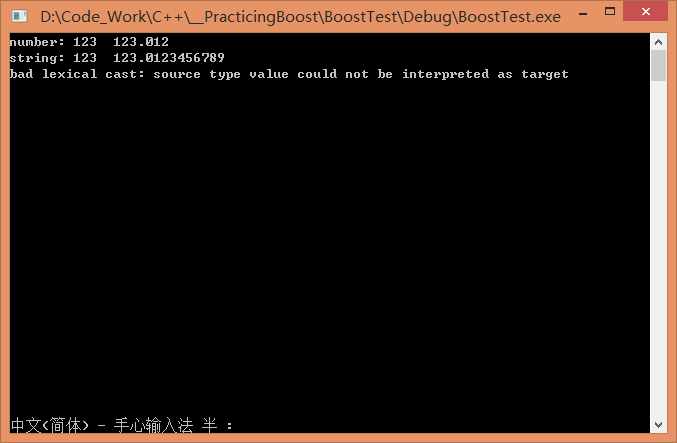
\includegraphics[width=14cm,clip]{BoostTest.png}
		 \end{figure}
		 
	\section{参考文献}\url{http://jingyan.baidu.com/article/11c17a2c765763f446e39dc1.html}	 

\newpage
\chapter{内存管理}
	\section{smart\_ptr}
	
		\subsection{RAII 机制(Resoource Acquisition Is Initialization)}
			为了管理内存等资源, C++程序员通查采
			用RAII机制-在使用资源的类的构造函数中申请资源,然后使用,最后在析构函数中释放资源。
			
			如果对象是声明的方式在栈上创建的-(一个局部对象),那么RAII机制会正常工作,当离开作用域时会自动销毁从而调用析构函数释放资源。
			
			如果对象是new 操作符在堆上创建的,那么它的析构函数不会自动调用,程序员必须明确的用对应的delete 操作符销毁它才能释放资源,这就存在资源泄漏的隐患-(如果因某些意外导致程序未能执行Delete语句,那么内存等资源就永久的丢失了)
			
			\subparagraph{内存泄漏的检查--异常}
				C++引入异常机制后,智能指针由一种技巧升级为一种非常重要的技术,因为如果没有智能指针,程序员必须保证new对象能在正确的时机delete,四处编写异常捕获代码以释放资源
				
			\subparagraph{内存泄漏的检查--智能指针}
				而智能指针则可以在推出作用域时-- 不管是正常流程离开或是因异常离开 --总能调用delete来析构在堆上动态分配的对象。也就是说是异常安全的
				
			\subparagraph{include boost/smart\_ptr.hpp}
				头文件包含
				
			\subparagraph{Assert 函数}
				include <assert.h>
				
				void assert( int expression );
				
				assert的作用是现计算表达式 expression,如果其值为假(即为0),那么它先向stderr打印一条出错信息,然后通过调用 abort 来终止程序运行
	
		\subsection{scoped\_ptr}
			它包装了new操作符在堆上分配的动态对象,能够保证动态创建的对象在任何时候都可以被正确删除,但是它的所有权更加严格,不能转让。一旦它获取了对象的管理权,你就无法再从它那里取回来。
			
			实质上是一个行为类似与指针的对象...
			
		\subsection{$\sharp$ scoped\_array}
			它很像scoped\_ptr, 它包装了new []操作符(不是单纯的new)在堆上分配的动态数组,为动态数组提供一个代理,\textit{保证可以正确的释放内存。}
			
			除非对性能有非常苛刻的要求,或者编译器不支持标准库(嵌入式),否则\textbf{不推荐使用}
			\begin{enumerate}[fullwidth,itemindent= 3em]
				\item 构造函数接受的指针p 必须是new[]的结果,而不是new表达式的结果
				\item 没有重载 *,->,即不可以使用这些操作符
				\item 析构函数使用delete[] 释放资源,而不是delete
				\item 提供operator[] 操作符重载,可以像数组使用下标
				\item 没有begin() end() 等类似容器的迭代操作函数
			\end{enumerate}
			
		\subsection{shared\_ptr}
			它包装了new操作符在堆上分配动态对象,实现了引用计数,可以被自由的拷贝和赋值,在任意地方共享它,当没有代码使用(引用计数为0时)它才删除被包装的动态分配的对象。 shared\_ptr 也可以安全地放到标准容器中,并弥补了auto\_ptr 因为转移语义而不能把指针作为STL容器元素的缺陷。
			
			作为STL容器元素的特点:
				\begin{enumerate}[fullwidth,itemindent = 3em]
					\item 必须可透过copy构造函数进行复制
					\item 必须可以透过assignment操作符完成赋值动作
					\item 必须可以透过析构函数完成销毁动作
				\end{enumerate}
			
			总结:\url{http://www.cnblogs.com/welkinwalker/archive/2011/10/20/2218804.html}
			
			理解共享:\url{http://www.cnblogs.com/TianFang/archive/2008/09/19/1294521.html}	
			
			\subparagraph{shared\_ptr 构造}:
				\begin{enumerate}[fullwidth,itemindent = 3em]
					\item shared\_ptr<T> ptr;  使用空参数构造函数构造
					\item shared\_ptr<T> ptr(new T());  直接从 new 操作符的返回值构造
					\item shared\_ptr<T> ptr2(ptr);  使用复制构造函数(或等号重载),从其它 shared\_ptr 的对象构造
					\item shared\_ptr<A> ptra( dynamic\_pointer\_cast<A>(ptrb) );此处假设 B 是 A 的子类
				\end{enumerate}
				
			\subparagraph{shared\_ptr 隐式拷贝构造||赋值}:
			\begin{lstlisting}
	shared_ptr<T> a(new T());
	shared_ptr<T> b(new T());
	a = b; // 此后 a 原先所指的对象会被销毁,b 所指的对象引用计数加 1
	
	//shared_ptr 的对象在构造之后,可以被赋予空值,此时使用的应该是 reset() 函数,如
	shared_ptr<T> a(new T());
	a.reset(); // 此后 a 原先所指的对象会被销毁,并且 a 会变成 NULL,前提是a没共享
	
	//理解共享
	class implementation
	{
	public:
		~implementation() { std::cout <<"destroying implementation\n"; }
		void do_something() { std::cout << "did something\n"; }
	};
	
	void test()
	{
		boost::shared_ptr<implementation> sp1(new implementation());
		std::cout<<"The Sample now has "<<sp1.use_count()<<" references\n";
		
		boost::shared_ptr<implementation> sp2 = sp1;
		std::cout<<"The Sample now has "<<sp2.use_count()<<" references\n";
		
		sp1.reset();
		std::cout<<"After Reset sp1. The Sample now has "<<sp2.use_count()<<" references\n";
		
		sp2.reset();
		std::cout<<"After Reset sp2.\n";
	}
	
	void main()
	{
		test();
	}
	
	/*
	该程序的输出结果如下:
	
	The Sample now has 1 references
	The Sample now has 2 references
	After Reset sp1. The Sample now has 1 references
	destroying implementation
	After Reset sp2. 
	*/			
			\end{lstlisting}
				
			\subparagraph{不要构造一个临时的shared\_ptr作为函数的参数}
			
			\subparagraph{make\_shared 工厂函数--消除显示的new调用}:
			
				消除new 与delete 不对称的强迫症患者,且效率比直接构造高,因为他使用的是右值的引用和move语义
				
			\subparagraph{共享容器 与 作为容器元素}:
				\begin{enumerate}[fullwidth,itemindent = 3em]
					\item shared\_ptr<list<T> > 共享容器 
					\item vector< shared\_ptr<T> >  元素 
				\end{enumerate}
				
			\subparagraph{定制删除器}:
			
				类似于 在初始化时指定析构函数,然后在退出时执行我们指定的函数...
				
				shared\_ptr<FILE> fp(fopen("./1.txt","r"), fclose);
				
				当离开作用域时,shared\_ptr 会自动调用fclose() 函数关闭文件
				
				\textit{shared\_ptr 的删除器在处理某些特殊资源时非常有用,它使得用户可以定制、扩展shared\_ptr 的行为,使得shared\_ptr不仅仅能够管理内存资源,而是成为一个“万能”的资源管理工具}
		\subsection{shared\_array}
			\subparagraph{共享数组}:
				即加了引用计数的共享数组...
		\subsection{weak\_ptr}
			像旁观者那样观测资源的使用情况.
			\subparagraph{构造}:
				weak\_ptr被设计为与shared\_ptr共同工作,可以从一个shared\_ptr或者另一个weak\_ptr对象构造,获得资源的观测权。但weak\_ptr没有共享资源,它的构造不会引起指针引用计数的增加。
			\subparagraph{使用}:
				使用weak\_ptr的成员函数use\_count()可以观测资源的引用计数,另一个成员函数expired()的功能等价于use\_count()==0,但更快,表示被观测的资源(也就是shared\_ptr的管理的资源)已经不复存在。
				weak\_ptr可以使用一个非常重要的成员函数lock()从被观测的shared\_ptr获得一个可用的shared\_ptr对象, 从而操作资源。但当expired()==true的时候,lock()函数将返回一个存储空指针的shared\_ptr.
			\subparagraph{示例}:
				\begin{lstlisting}
	shared_ptr<int> sp(new int(10));
	assert(sp.use_count() == 1);
	
	weak_ptr<int> wp(sp); //从shared_ptr创建weak_ptr
	assert(wp.use_count() == 1);
	
	if (!wp.expired())//判断weak_ptr观察的对象是否失效
	{
		shared_ptr<int> sp2 = wp.lock();//获得一个shared_ptr
		*sp2 = 100;
		assert(wp.use_count() == 2);
	}
	assert(wp.use_count() == 1);			
				\end{lstlisting}
	\section{pool 内存池管理}
			\subparagraph{参考文献}:\verb|http://blog.csdn.net/sndaxdrs/article/details/6175615|
\newpage
\chapter{实用工具}


\newpage
\chapter{字符串与文本处理}


\newpage
\chapter{容器与数据结构}
\section{在容器或变量中存储任意值}
	\subsection{使用Boost.Any 库}
	\begin{lstlisting}
	#include<boost/any.hpp>
	int main()
	{
		std::vector<boost::any>some_values;
		some_values.push_back(10);
		const char* c_str = "Hello there";
		some_values.push_back(c_str);
		some_values.push_back(std::string("Wow!"));
		
		std::string& s = 
			boost::any_cast<std::string&>(some_values.back()); //强制转化最后一个元素,因为程序员知道他是什么类型
		
		s += "That's great!"
		std::cout<< s <<endl;	
		return 0;
	}
	
	//可以使用两种方法从 boost::any 获得值
	boost::any variable(std::string("Hello"));
	
	//#1:如果变量的实际值不是一个std::string,以下方法会抛出一个boost::bad_any_cast 异常
	std::string s1 = boost::any_cast<std::string>(variable);
	
	//#2:如果变量的实际值不是一个std::string 将返回一个nullptr 指针
	std::string* s2 = boost::any_cast<std::string>(&variable);
	\end{lstlisting}
	
		\paragraph{特点}
		\begin{itemize}
			\item 这种灵活性总是要付出代价的;
			\item 为boost::any 的实例赋值构造、值构造、复制赋值和赋值 将调用一个动态内存(堆)分配函数;
			\item 所有类型的强制装换需要获得运行时的类型信息(Run Time Tyoe Information(RTTI));
			\item boost::any 大量使用虚函数,所以性能就会受限;
		\end{itemize}
		
	\subsection{使用Boost.Variant 库}
		实质是类型安全的Union
	\begin{lstlisting}
	#include<boost/variant.hpp>
	int main()
	{
		typedef boost::variant<int, const char*,std::string>my_var_t;
		
		std::vector<my_var_t>some_values;
		some_values.push_back(10);
		const char* c_str = "Hello there";
		some_values.push_back(c_str);
		some_values.push_back(std::string("Wow!"));
		
		std::string& s = 
		boost::get<std::string>(some_values.back()); //强制转化最后一个元素,因为程序员知道他是什么类型
		
		s += "That's great!"
		std::cout<< s <<endl;	
		return 0;
	}
	
	//可以使用两种方法从 boost::variant 获得值
	boost::variant<int,std::string> variable(0);
	
	//#1:如果变量的实际值不是一个int型,以下方法会抛出一个boost::bad_any_cast 异常
	int s1 = boost::get<int>(variable);
	
	//#2:如果变量的实际值不是一个int型, 将返回一个nullptr 指针
	int* s2 = boost::get<int>(&variable);
	\end{lstlisting}
	
		\paragraph{特点}
		\begin{itemize}
			\item 变量通常不再堆中分配内存
			\item 不需要启用RTTI
			\item 执行速度非常快
		\end{itemize}
\newpage
\chapter{算法}


\newpage
\chapter{数字与数学}


\newpage
\chapter{操作系统相关}


\newpage
\chapter{Asio 组件}



\newpage
\chapter{测试}
	\section{单元测试}
		复杂的 C/C++ 代码中很可能有 bug,到代码编写完成之后再来测试就像大海捞针。比较谨慎的办法是,在编写各个代码段时,针对特定的区域(例如,一些包含大量计算的 C 函数或声明队列等数据结构的 C++ 类),添加专门的小测试(单元测试),以在编写代码的同时进行测试。按这种方式构建的回归测试套件包含一套单元测试和一个测试驱动程序,这个程序运行测试并报告结果
		
	\subsection{为特定的函数或类生成测试}
		对于文本编辑器这样复杂的代码,外部测试者无法生成针对特定例程的测试 — 测试者不太了解内部代码组织。\textbf{Boost 的优势就在于白箱测试} :由开发人员编写测试,对类和函数进行语义检查。这个过程极其重要,因为代码以后的维护者可能会破坏原来的逻辑,这时单元测试就会失败。通过使用白箱测试,常常很容易找到出错的地方,不必使用调试器。
		
		请考虑以下的简单字符串类。这个类并不健壮,我们使用 Boost 来测试它
			\begin{lstlisting}
	// 清单 1. 简单的字符串类
	#ifndef _MYSTRING
	#define _MYSTRING
	
	class mystring { 
		char* buffer; 
		int length;
	public: 
		void setbuffer(char* s) { buffer = s; length = strlen(s); } 
		char& operator[ ] (const int index) { return buffer[index]; }
		int size( ) { return length; }
	}; 
	
	#endif
			\end{lstlisting}
		
		与字符串相关的一些典型的检查,会验证空字符串的长度是否为 0,访问范围超出索引是否导致错误消息或异常,等等。清单 2 给出了一些值得为任何字符串实现创建的测试。要想运行 清单 2 中的源代码,只需用 g++(或任何符合标准的 C++ 编译器)编译它。注意,不需要单独的主函数,代码也不使用任何链接库:作为 Boost 一部分的 \verb|unit_test.hpp| 头文件中包含所需的所有定义。
			\begin{lstlisting}
	// 清单 2. 字符串类的单元测试
	#define BOOST_TEST_MODULE stringtest
	#include <boost/test/included/unit_test.hpp>
	#include "./str.h"
	
	BOOST_AUTO_TEST_SUITE (stringtest) // name of the test suite is stringtest
	
	BOOST_AUTO_TEST_CASE (test1)
	{
		mystring s;
		BOOST_CHECK(s.size() == 0);
	}
	
	BOOST_AUTO_TEST_CASE (test2)
	{
		mystring s;
		s.setbuffer("hello world");
		BOOST_REQUIRE_EQUAL ('h', s[0]); // basic test 
	}
	
	BOOST_AUTO_TEST_SUITE_END( )			
			\end{lstlisting}
			\begin{itemize}
				\item \verb|BOOST_AUTO_TEST_SUITE| 和 \verb|BOOST_AUTO_TEST_SUITE_END| 宏\textbf{分别表示测试套件的开头和结尾}
				\item \textbf{各个测试放在这两个宏之间},从这一点来看,这些宏的语义很像 C++ 名称空间
				\item \textbf{每个单元测试用} \verb|BOOST_AUTO_TEST_CASE| 宏来定义
			\end{itemize}
			清单 3 给出了 清单 2 中代码的输出。
			\begin{lstlisting}
	// 清单3.清单 2 中代码的输出
	[arpan@tintin] ./a.out
	Running 2 test cases...
	test.cpp(10): error in "test1": check s.size() == 0 failed
	
	*** 1 failure detected in test suite "stringtest"
			\end{lstlisting}
	
	\subsection{Boost 测试工具}
		Boost 有一整套测试工具,基本上可以说它们是用于验证表达式的宏。测试工具的三个主要类别是 \verb|BOOST_WARN|、\verb|BOOST_CHECK| 和 \verb|BOOST_REQUIRE|。  
		
		 对于\verb|BOOST_CHECK|,即使断言失败,测试仍然继续执行;而对于\verb|BOOST_REQUIRE|,认为这是严重的错误,测试会停止
		 
		 清单 4 使用一个简单的 C++ 片段展示了这些工具类别之间的差异
		 \begin{lstlisting}
	// 清单 4. 使用 Boost 测试工具的三个变体
	#define BOOST_TEST_MODULE enumtest
	#include <boost/test/included/unit_test.hpp>
	
	BOOST_AUTO_TEST_SUITE (enum-test) 
	
	BOOST_AUTO_TEST_CASE (test1)
	{
		typedef enum {red = 8, blue, green = 1, yellow, black } color;
		color c = green;
		BOOST_WARN(sizeof(green) > sizeof(char));
		BOOST_CHECK(c == 2); 
		BOOST_REQUIRE(yellow > red); 
		BOOST_CHECK(black != 4);
	}
	
	BOOST_AUTO_TEST_SUITE_END( )
		 \end{lstlisting}
		 第一个 \verb|BOOST_CHECK| 会失败,第一个 \verb|BOOST_REQUIRE| 也是如此。但是,当 \verb|BOOST_REQUIRE| 失败时,代码退出,所以不会到达第二个 \verb|BOOST_CHECK|
		 
		 清单 5 显示了 清单 4 中代码的输出。
		 \begin{lstlisting}
	\\ 清单 5. 理解 BOOST_REQUIRE 和 BOOST_CHECK 之间的差异
	[arpan@tintin] ./a.out
	Running 1 test case...
	e2.cpp(11): error in "test1": check c == 2 failed
	e2.cpp(12): fatal error in "test1": critical check yellow > red failed
	
	*** 2 failures detected in test suite "enumtest"
		 \end{lstlisting}
		 同样,如果需要针对特定情况检查某些函数或类方法,最容易的方法是创建一个新测试,并使用参数和期望值调用这个例程。清单 6 提供了一个示例。
		 \begin{lstlisting}
	\\ 清单 6. 使用 Boost 测试检查函数和类方法
	BOOST_AUTO_TEST(functionTest1) 
	{
		BOOST_REQUIRE(myfunc1(99, ‘A’, 6.2) == 12);
		myClass o1(“hello world!\n”);
		BOOST_REQUIRE(o1.memoryNeeded( ) < 16);
	}
		 \end{lstlisting}
		 \subsection{模式匹配}
		 
		 \subsection{浮点比较}
			 回归测试中最棘手的检查之一是浮点比较。请看一下 清单 8,看起来没什么问题 — 至少从表面看是这样
			 \begin{lstlisting}
	// 清单 8. 无效的浮点比较
	#define BOOST_TEST_MODULE floatingTest
	#include <boost/test/included/unit_test.hpp>
	#include <cmath>
	
	BOOST_AUTO_TEST_SUITE ( test ) 
	
	BOOST_AUTO_TEST_CASE( test )
	{
	float f1 = 567.0102;
	float result = sqrt(f1); // this could be my_sqrt; faster implementation
	// for some specific DSP like hardware
	BOOST_CHECK(f1 == result * result);  
	}
	
	BOOST_AUTO_TEST_SUITE_END( ) 
			 \end{lstlisting}
			 
			 运行这个测试时,尽管使用的是作为标准库一部分提供的 sqrt 函数,\verb|BOOST_CHECK| 宏仍然会失败。什么地方出错了?浮点比较的问题在于精度 — f1 和 result*result 在小数点后面的几位不一致。为了解决这个问题,Boost 测试实用程序提供了 \verb|BOOST_WARN_CLOSE_FRACTION|、\verb|BOOST_CHECK_CLOSE_FRACTION| 和 \verb|BOOST_REQUIRE_CLOSE_FRACTION| 宏。要想使用这三个宏,必须包含预定义的 Boost 头文件 \verb|floating_point_comparison.hpp|。这三个宏的语法是相同的,所以本文只讨论 check 变体(见 清单 9)
			 \begin{lstlisting}
	// 清单 9. BOOST_CHECK_CLOSE_FRACTION 宏的语法
	BOOST_CHECK_CLOSE_FRACTION (left-value, right-value, tolerance-limit);
	
	// 有效的浮点比较
	#define BOOST_TEST_MODULE floatingTest
	#include <boost/test/included/unit_test.hpp>
	#include <boost/test/floating_point_comparison.hpp>
	#include <cmath>
	
	BOOST_AUTO_TEST_SUITE ( test ) 
	
	BOOST_AUTO_TEST_CASE( test )
	{
		float f1 = 567.01012;
		float result = sqrt(f1); // this could be my_sqrt; faster implementation
		// for some specific DSP like hardware
		BOOST_CHECK_CLOSE_FRACTION (f1, result * result, 0.0001);  
	}
	
	BOOST_AUTO_TEST_SUITE_END( )
	
	// 这段代码运行正常。现在,把公差限制改为 0.0000001
	由于超过公差限制,比较失败
	[arpan@tintin] ./a.out
	Running 1 test case...
	sq.cpp(18): error in "test": difference between f1{567.010132} and 
	result * result{567.010193} exceeds 1e-07
	
	*** 1 failure detected in test suite "floatingTest"
			 \end{lstlisting}
			 生产软件中另一个常见的问题是比较 double 和 float 类型的变量。\verb|BOOST_CHECK_CLOSE_FRACTION| 的优点是它不允许进行这种比较。这个宏中的左值和右值必须是相同类型的 — 即要么是 float,要么是 double。在 清单 12 中,如果 f1 是 double,而 result 是 float,在比较时就会出现错误。如下所示:
			 \begin{lstlisting}
	\\ 错误:BOOST_CHECK_CLOSE_FRACTION 的左值和右值参数的类型不同
	[arpan@tintin] g++ sq.cpp -I/u/c/lib/boost
	/u/c/lib/boost/boost/test/test_tools.hpp: 
		In function 
			`bool boost::test_tools::tt_detail::check_frwd(Pred, 
			const boost::unit_test::lazy_ostream&, 
			boost::test_tools::const_string, size_t, 
			boost::test_tools::tt_detail::tool_level, 
			boost::test_tools::tt_detail::check_type, 
			const Arg0&, const char*, 
			const Arg1&, const char*, const Arg2&, const char*) 
			[with Pred = boost::test_tools::check_is_close_t, Arg0 = double, 
			Arg1 = float, Arg2 = boost::test_tools::fraction_tolerance_t<double>]':
		sq.cpp:18:   instantiated from here
		/u/c/lib/boost/boost/test/test_tools.hpp:523: error: no match for call to
			`(boost::test_tools::check_is_close_t) (const double&, const float&, 
				const boost::test_tools::fraction_tolerance_t<double>&)'
			 \end{lstlisting}
			 
		 \subsection{定制的断言支持}
			 Boost 测试工具验证 Boolean 条件。可以通过扩展测试工具支持更复杂的检查 — 例如,判断两个列表的内容是否相同,或者某一条件对于向量的所有元素是否都是有效的。还可以通过扩展 \verb|BOOST_CHECK| 宏执行定制的断言检查。下面对用户定义的 C 函数生成的列表内容执行定制的检查:检查结果中的所有元素是否都大于 1。定制检查函数需要返回 \verb|boost::test_tools|
			 \verb|::predicate_result| 类型。清单 13 给出了详细的代码。
			 \begin{lstlisting}
	// 清单 13. 使用 Boost 测试工具验证复杂的断言
	#define BOOST_TEST_MODULE example
	#include <boost/test/included/unit_test.hpp>
	
	boost::test_tools::predicate_result validate_list(std::list<int>& L1)
	{ 
		std::list<int>::iterator it1 = L1.begin( );
		for (; it1 != L1.end( ); ++it1) 
		{ 
			if (*it1 <= 1) return false; 
		}
		return true;
	}
	
	BOOST_AUTO_TEST_SUITE ( test ) 
	
	BOOST_AUTO_TEST_CASE( test )
	{
		std::list<int>& list1 = user_defined_func( );
		BOOST_CHECK( validate_list(list1) );
	}
	
	BOOST_AUTO_TEST_SUITE_END( )
			 \end{lstlisting}
			 \verb|predicate_result| 对象有一个隐式的构造函数,它接受一个 Boolean 值,因此即使 \verb|validate_list| 的期望类型和实际返回类型不同,代码仍然会正常运行。
			 还有另一种用 Boost 测试复杂断言的方法:\verb|BOOST_CHECK_PREDICATE| 宏。这个宏的优点是它不使用 \verb|predicate_result|。但缺点是语法有点儿粗糙。用户需要向 \verb|BOOST_CHECK_PREDICATE| 宏传递函数名和参数。清单 14 的功能与 清单 13 相同,但是使用的宏不同。注意,\verb|validate_result| 的返回类型现在是 Boolean
			\begin{lstlisting}
	// 清单 14. BOOST_CHECK_PREDICATE 宏
	#define BOOST_TEST_MODULE example
	#include <boost/test/included/unit_test.hpp>
	
	bool validate_list(std::list<int>& L1)
	{ 
		std::list<int>::iterator it1 = L1.begin( );
		for (; it1 != L1.end( ); ++it1) 
		{ 
			if (*it1 <= 1) return false; 
		}
		return true;
	}
	
	BOOST_AUTO_TEST_SUITE ( test ) 
	
	BOOST_AUTO_TEST_CASE( test )
	{
		std::list<int>& list1 = user_defined_func( );
		BOOST_CHECK_PREDICATE( validate_list, list1 );
	}
	
	BOOST_AUTO_TEST_SUITE_END( )
			\end{lstlisting}
		 \subsection{在一个文件中包含多个测试套件}
			 可以在一个文件中包含多个测试套件。文件中定义的每个测试套件必须有一对 \verb|BOOST_AUTO_TEST_SUITE|... \verb|BOOST_AUTO_TEST_SUITE_END| 宏。清单 15 给出了在同一个文件中定义的两个测试套件。在运行回归测试时,用预定义的 \verb|–log_level=test_suite| 选项运行可执行程序。在 清单 16 中可以看到,使用这个选项生成的输出很详细,有助于进行快速调试。
			 \begin{lstlisting}
	// 清单 15. 使用一个文件中的多个测试套件
	#define BOOST_TEST_MODULE Regression
	#include <boost/test/included/unit_test.hpp>
	
	typedef struct {
		int c;
		char d;
		double e;
		bool f;
	} Node;
	
	typedef union  {
		int c;
		char d;
		double e;
		bool f;
	} Node2;
	
	BOOST_AUTO_TEST_SUITE(Structure)
	
	BOOST_AUTO_TEST_CASE(Test1)
	{
		Node n;
		BOOST_CHECK(sizeof(n) < 12);
	}
	
	BOOST_AUTO_TEST_SUITE_END()
	
	BOOST_AUTO_TEST_SUITE(Union)
	
	BOOST_AUTO_TEST_CASE(Test1)
	{
		Node2 n;
		BOOST_CHECK(sizeof(n) == sizeof(double));
	}
	
	BOOST_AUTO_TEST_SUITE_END()
	
	// --------->Result 
	// 用 –log_level 选项运行多个测试套件
	[arpan@tintin] ./a.out --log_level=test_suite
	Running 2 test cases...
	Entering test suite "Regression"
	Entering test suite "Structure"
	Entering test case "Test1"
	m2.cpp(23): error in "Test1": check sizeof(n) < 12 failed
	Leaving test case "Test1"
	Leaving test suite "Structure"
	Entering test suite "Union"
	Entering test case "Test1"
	Leaving test case "Test1"
	Leaving test suite "Union"
	Leaving test suite "Regression"
	
	*** 1 failure detected in test suite "Regression"
			 \end{lstlisting}
	\section{回归测试}
		回归测试是\textbf{指修改了旧代码后,重新进行测试以确认修改没有引入新的错误或导致其他代码产生错误}。自动回归测试将大幅降低系统测试、维护升级等阶段的成本。回归测试作为软件生命周期的一个组成部分,在整个软件测试过程中占有很大的工作量比重,软件开发的各个阶段都会进行多次回归测试。在渐进和快速迭代开发中,新版本的连续发布使回归测试进行的更加频繁,而在极端编程方法中,更是要求每天都进行若干次回归测试。因此,通过选择正确的回归测试策略来改进回归测试的效率和有效性是很有意义的
		
		\subparagraph{观点}:
			\begin{itemize}
				\item 回归测试是指重复以前的全部或部分的相同测试
				\item 新加入测试的模组,可能对其他模组产生副作用,故须进行某些程度的回归测试
				\item 回归测试的重心,以关键性模组为核心
			\end{itemize}
	\section{参考文献}
		boost 测试:\url{http://www.ibm.com/developerworks/cn/aix/library/au-ctools1_boost/}
		
		回归测试:baidu 百科	   
\end{document} 
 		    